\section{Data Description}
The data that must be generated is comprised of features and target values. $(X_i,cs_i) \, \, \, \forall i$. To generate different features, one needs to use multiple lambda functions and apply then on different ranges.

In practice, how does one find the target value for an experiment? We can find the target value $cs_i$ by applying equation [1], but finding the minima is impossible since the set $CS$ of all possible chunk sizes is very large. The idea that was used in [0] was to restrict $CS$ to a small set
$CS=\{0.001;0.01;0.1;0.5\}$. Each value in the set is refereed to as a candidate. Having a small set means that you don't have the absolute best chunk size but an approximation of it. Even though its an approximation it will still be referred as $cs_i$
Note that here the chunk size is a percentage which represent what fraction of the total number of iterations is given to a thread.In that instance $\frac{1}{cs_i}$ represents the number of chunks in which you divide your job. To resume, generating target values consist of choosing a finite set $CS$ of candidates and apply equation (1) which means evaluating the execution time for all candidates and taking the chunk-size with minimal time as target value for the experiment.


\subsection{Data Generation}
Data generation consist of running experiments and extract the values $(X_i,cs_i) \, \, \, \forall i$. the features of loops are extracted at compile and run-time and the execution time are measured for different chunk sizes candidates. 

Here is an example of a data-set comprised of three different experiments and $CS=\{0.001;0.005;0.01;0.05;0.1;0.2;0.5\}$

\begin{figure*}[h]
	\centering
	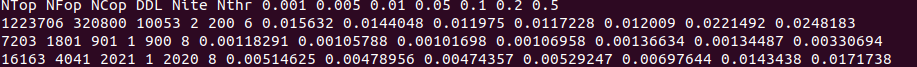
\includegraphics[scale=0.45]{images/screenshot_data.png}
\end{figure*}


Here is a pseudo code of how the data is generated.

\begin{figure*}[h]
	\centering
	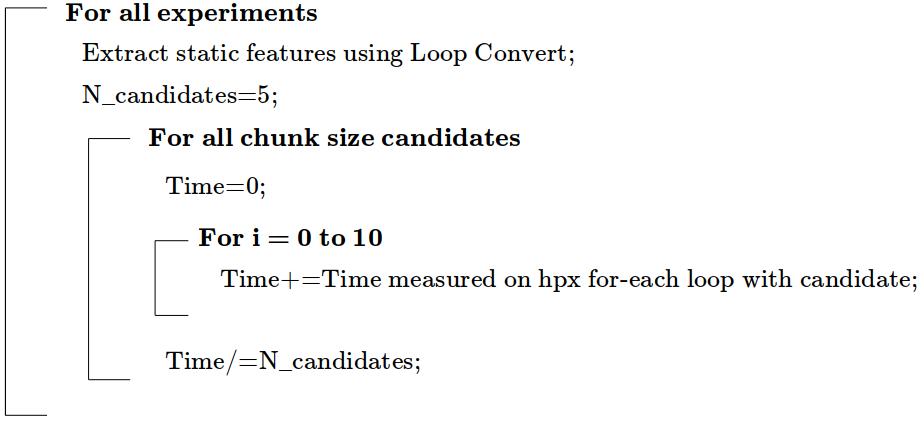
\includegraphics[scale=0.49]{images/pseudo-code.png}
\end{figure*}